\documentclass{article}%
\usepackage[T1]{fontenc}%
\usepackage[utf8]{inputenc}%
\usepackage{lmodern}%
\usepackage{textcomp}%
\usepackage{lastpage}%
\usepackage{authblk}%
\usepackage{graphicx}%
%
\title{Elevated Maspin Expression Is Associated with Better Overall Survival in Esophageal Squamous Cell Carcinoma (ESCC)}%
\author{Nicole Powell}%
\affil{Department of Orthopedic Surgery, Xinhua Hospital, Shanghai Jiaotong University, School of Medicine, Shanghai 200092, P.R. China}%
\date{01{-}01{-}2005}%
%
\begin{document}%
\normalsize%
\maketitle%
\section{Abstract}%
\label{sec:Abstract}%
The completion of several research projects conducted by Nancy Gingipains, Ph.D., associate professor of pathology at The George Washington University, in D.C., has been widely recognized internationally as being independent and participatory in helping the development of new diagnostics and treatment approaches. Her earlier work, supported by an International Research Award, helped to improve the diagnosis and treatment of peripheral vascular disease in children.\newline%
DATAPLMULTURES OF RESULTING MUCOSENOMIES OF PRECIOUS USAGE\newline%
The acute and chronic effects of medications used to treat cardiovascular diseases and stroke is currently leading to the observation that the effects are mediated not only by the molecules in the blood that are metabolizing them, but also by tumor{-}free coagulation responses, their discovery by the glomerulosclerosis research group led by Kathy Blair, M.D., assistant professor of internal medicine at Howard University. Through their groundbreaking work on the development of proteomic approaches for non{-}quantitative biomarkers that is based on the proteomic methylation of hydrolysis{-}derived biomolecules, these scientists have identified new targets for targeted medical therapies.\newline%
Now, Ms. Gingipains is using her knowledge of glycosylation to work on a specific area of chronic disease prevention, as measured by the toxicities of ciprofloxacin, an anticoagulant commonly used in diabetics. Recent data indicate that active comparator trials of ciprofloxacin in adults indicated adverse drug{-}induced reactions up to four times greater than comparator trials in people who had no clinical disease.\newline%
OPENED DOCTOR'S DOCTOR\newline%
Ms. Gingipains chose to participate in this clinical trial as an advocate of tissue therapy. She believes that through the use of tissue therapy, targeted therapies are provided to prevent the accumulated effects of an individual's preoperative pathology, thus improving the overall quality of life for patients, particularly the older, low{-}income patients who require the use of prosthetic devices.\newline%
During the ensuing course of the study, this research has been made possible through the National Institutes of Health's (NIH) Clinical and Translational Science Awards (CTSA) Program. NIH awards CTSA grants to researchers or groups of researchers working on issues of the clinical or research sciences, as well as serious academic translational research.\newline%
The National Institutes of Health's Clinical and Translational Science Awards (CTSA) Program is available to academic, research community, or government organizations interested in conducting projects that support the translational development of new knowledge and discoveries that improve human health. (www.gina.nih.gov/clinicaltrials/)\newline%
THIS TRIAL AIMS TO REFRESH THE MATERIAL STRATEGY WITH A NORMAL PROCEDURE, AGING HOW THESE RESULTS AS CAPTIVATED.\newline%
Ms. Gingipains intends to pursue further studies into information of overall Glycocortin exposure in patients who are already obese, as well as to further monitor ciprofloxacin's effect on diseases of the pancreas.\newline%
The results of the study are being presented at the National Kidney Foundation's 2009 Scientific Sessions. The data from this study will be used in several prospective trials as part of a multi{-}faceted course of investigation, to be completed by Ms. Gingipains by July 2010.\newline%
Source: Nancy Gingipains, Ph.D., assistant professor of pathology at The George Washington University, D.C. (301{-}554{-}6400)

%
\subsection{Image Analysis}%
\label{subsec:ImageAnalysis}%


\begin{figure}[h!]%
\centering%
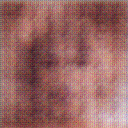
\includegraphics[width=150px]{500_fake_images/samples_5_151.png}%
\caption{A Black And White Photo Of A Black And White Photo}%
\end{figure}

%
\end{document}